\documentclass[11pt]{article}
\usepackage[a4paper,margin=24mm]{geometry}
\usepackage{amsmath,amssymb,booktabs,graphicx,microtype}
\usepackage[hidelinks]{hyperref}
\usepackage{array}
\title{Answer Consistency under Quantization:\\
A Controlled Study with Exact Input Transformations}
\author{Working research draft\\Author and affiliation to be confirmed}
\date{8 November 2026}
\begin{document}
\maketitle

\begin{abstract}
Weight quantization can change how a language model answers equivalent
presentations of the same problem. We study this behavior with executable
answer oracles and explicit transport of displayed options to canonical
answer identities. A two-model pilot illustrates why agreement alone is
insufficient: four-bit SmolLM2 becomes more consistent while losing accuracy.
We compare scale-only teacher distillation with a paired invariance objective,
holding input exposure and optimization updates fixed, with three fit seeds
and 1,152 independent evaluation bases per model. Paired calibration reduces
consistency on held-out single transformations for both models. Qwen's joint
correctness improves by 2.04--11.50 percentage points, while Smol's changes
range from $-15.62$ to $+4.25$ points. On compositions withheld from both
fitting and development selection, Qwen's consistency rises by
14.71--20.62 points, but Smol's changes range from $-5.25$ to $+9.11$.
The effects depend on model and fit seed; they do not support a general
preservation benefit. The released numerical RTN study separates useful
agreement, wrong agreement, and fidelity to the full-precision teacher.
\end{abstract}

\section{Introduction}
Two answers can agree because a model follows the same reasoning, because
it repeats the same mistake, or because it favors a displayed option.
Quantization can change all three behaviors. Average task accuracy does not
identify which individual predictions changed, while consistency by itself
does not identify correct reasoning. A useful evaluation must retain the
identity of an answer across transformations and distinguish jointly correct
pairs from pairs that consistently select a wrong answer.

This distinction is particularly concrete in multiple-choice tasks.
Permuting choices changes the correct displayed letter while preserving the
underlying answer. Renaming entities or reordering independent facts should
preserve that answer as well. Comparing raw letters across an option
permutation would therefore measure the wrong relation. We instead store an
explicit display-to-canonical bijection and recompute every correctness
label from an executable oracle.

Behavior-aware quantization is established. FidelityQ targets predictive
fidelity, DPQ targets uncertainty preservation, and EAQuant targets
answer-supporting evidence \cite{fidelityq,dpq,eaquant}. KernelQuant already
preserves relations among calibration representations \cite{kernelquant}.
Our study consequently does not claim that preserving behavior or relations
during quantization is new. We test a narrower question: does a loss based
on known semantic input correspondences improve held-out correspondence
beyond giving a quantized model exactly the same transformed inputs without
that paired loss?

The study provides an exact procedural evaluation with separated calibration,
development, pilot, and final bases, and a matched comparison of five
scale-calibration objectives. It evaluates accuracy, teacher prediction
fidelity, joint correctness, and consistently wrong agreement alongside
consistency. These controls make a negative outcome informative: generic
calibration, data augmentation, or a trivial option preference may account
for an apparent invariance gain.

\section{Related work and scope of novelty}
Consistency regularization across augmented inputs is established in both
language and vision \cite{uda}. AugMix explicitly uses Jensen--Shannon
divergence across original and augmented predictions \cite{augmix}.
Neither the divergence nor invariance training is introduced here.
Our comparison applies these ingredients to frozen-code quantization scales
with exact option transport and a controlled information boundary.

Output matching and scale optimization are prior methods rather than
contributions of this study. OSTQuant uses learned transformations and
teacher supervision \cite{ostquant}; RoleQ includes next-token distillation
of scales with frozen integer codes \cite{roleq}. FPTQuant studies internal
function-preserving transformations \cite{fptquant}, a different use of
symmetry from transforming the question presented to a model.
Prompt-sensitivity changes under quantization are also known
\cite{deceptive}. A separate audit studies agreement in stochastic model
panels \cite{panels}; our relation compares explicitly mapped presentations
of one base problem. Exact transformation testing is not introduced here as
a new general testing methodology. Correctness Agreement also measures the
intersection of correct decisions between full-precision and quantized models
on identical inputs \cite{illusion}. Joint correctness and the observation
that equal accuracy can hide different decisions are established; our pairs
instead compare distinct mapped presentations under the same model.

KernelQuant is an especially relevant alternative: its calibration preserves
cosine kernels among representations \cite{kernelquant}. Our kernel-loss
control uses the same end-to-end optimization budget as the other controls,
but it is an adaptation at the final hidden representation, not a
reproduction of KernelQuant's layerwise scale search, error compensation,
rotation, and activation clipping. The bounded literature search found no
direct match for the exact semantic-pair calibration and held-out evaluation
contract used here. This is a statement about the searched sources, not
proof of priority.

\section{Exact tasks and correspondence}
We generate arithmetic evaluation, Boolean-assignment selection, and directed
acyclic graph questions. Each question has four distinct options and one
correct canonical option, verified by integer arithmetic, exhaustive Boolean
evaluation, or directed breadth-first search. Arithmetic expressions use
addition, subtraction, and multiplication with explicit parentheses. Boolean
questions ask which complete assignment makes an expression true. Graph
questions ask for a reachable candidate or one at an exact shortest distance.

The transformations are a seeded nonidentity option permutation, a consistent
entity renaming, and, for Boolean/graph questions, reordering independent
assignment facts or directed edges. Arithmetic order is not changed.
For final evaluation only, we also compose option permutation with renaming,
and with renaming and fact order where supported. Compositions reuse the
exact component maps rather than sampling new ones.

Calibration and development each contain 128 bases per task family; the
pilot contains 64, the final split 256, and a separate structural holdout 128.
Variants of a base always remain in the same split. Exact normalized
structures are disjoint across splits, excluding distractor choices and
arithmetic character names from the identity key. This boundary does not
deduplicate arbitrary Boolean logical equivalence or graph isomorphism.
Deterministic rejection resolves duplicate candidates, and the manifest
retains candidate counts and rejection reasons.

The structural holdout uses five or six arithmetic operations rather than
two or three, five Boolean assignment variables rather than three or four
with a maximum expression depth of three rather than two, and eight to ten
graph nodes rather than five to seven. A Boolean expression need not use
every assignment variable, so this split does not guarantee a strict
increase in logical difficulty for every question.

For base $i$, presentation $t$, and displayed option $j$, let $m_{it}(j)$
denote the canonical option identity. With the official chat template, the
model produces next-token option logits $z_{itj}$ for the verified single
tokens A--D. We predict
\[
 \widehat a_{it}=m_{it}\!\left(\arg\max_j z_{itj}\right).
\]
Probabilities are computed in FP32; predictions use logits directly, avoiding
artificial ties from BF16 softmax rounding. For paired losses, the four-option
probability vector is transported by
$p^{\mathrm{can}}_{it,m_{it}(j)}=\operatorname{softmax}(z_{it})_j$.
This is constrained next-token scoring, not evaluation of free generation.

Let $Y_{it}$ indicate correctness under the exact oracle. For each
non-original presentation define
\[
 C_{it}=\mathbf{1}[\widehat a_{i0}=\widehat a_{it}],\qquad
 J_{it}=Y_{i0}Y_{it},\qquad
 W_{it}=C_{it}(1-Y_{i0}).
\]
Here $C$ is consistency, $J$ joint correctness, and $W$ consistently wrong
agreement. A unique correct canonical option makes $J$ a subset of $C$.
We first average over the available variants of each base, then over bases.
The primary held-out endpoint uses entity renaming and fact order only;
compositions and structural holdout are reported separately. Pointwise
teacher fidelity is the fraction of canonical predictions matching BF16
on the same input.

Consistency change necessarily involves pointwise prediction change.
If $F_{i0}$ and $F_{it}$ indicate BF16-to-quantized answer flips, then
$|C^{q}_{it}-C^{f}_{it}|\leq F_{i0}+F_{it}$. We use this elementary bound
as an implementation diagnostic, not a novel theorem or an independent
failure mechanism.

\section{Quantization and matched calibration}
The reference models use BF16. Every transformer linear weight except the
embedding and output head is quantized independently within input-column
groups of 128, including tail groups. For bit width $b$, the RTN scale is
$s_g=\max_{k\in g}|w_k|/(2^{b-1}-1)$ and codes are
\[
 q_k=\operatorname{clip}\!\left(
 \operatorname{round}(w_k/s_g),-2^{b-1},2^{b-1}-1\right).
\]
All-zero groups reconstruct exactly zero. The pilot evaluates W8, W4, and W3.
The calibration comparison uses W4. Integer codes, pretrained weights,
biases, embeddings, output head, and normalization gains remain fixed.
Only positive group scales are learned:
\[
 \widetilde s_g=s_g\exp(\delta_g),\qquad \delta_g=0\text{ initially}.
\]
This stable relative parameterization exactly reproduces RTN at initialization.
Weights are reconstructed and rounded to BF16 during forward passes.
The experiment establishes numerical weight-quantization behavior, not
packed-format deployment parity, memory savings, or inference acceleration.

\subsection{Objectives and supervision}
The teacher cache contains complete final next-token vocabulary logits and
the final normalized hidden vector for each calibration original and its
option-permuted partner. No gold answer labels are training targets.
All optimized methods share the temperature-one loss
$\mathcal L_{\mathrm{KD}}=\operatorname{mean}_x
 \mathrm{KL}(P_f(\cdot\mid x)\Vert P_q(\cdot\mid x))$ over the full vocabulary.
They differ only in input presentation or the extra regularizer:
\begin{enumerate}
\item Original-only KD duplicates each original, keeping eight prompt rows
per update.
\item Augmented KD uses each original and its option-permuted partner
independently.
\item Paired calibration adds $\lambda$ times the mean Jensen--Shannon
divergence between the canonically transported four-option distributions
of each true pair.
\item Random-pair calibration adds the same loss after shifting the variants
cyclically to different bases in the shuffled minibatch.
\item The kernel control adds $\lambda B^{-2}\|H_fH_f^\top-H_qH_q^\top\|_F^2$,
where $H$ contains the unit-normalized final hidden vectors of the same
$B=8$ prompt rows, with $H\in\mathbb{R}^{B\times d}$ and model hidden width $d$.
\end{enumerate}
The paired objective imposes extra invariance. An inconsistent teacher can
therefore disagree with its regularizer; this is not exact preservation of
every teacher relation. Accuracy, fidelity, and consistently wrong agreement
are required to interpret any consistency gain.

Every scale-calibration fit starts from identical RTN scales and uses AdamW with learning rate
0.001, betas $(0.9,0.999)$, no weight decay, gradient-norm clipping at one,
and zero dropout. One shuffled epoch consists of 96 updates with four bases
and eight prompts per update, covering 384 bases and 768 prompts.
All loss computations and scale parameters are FP32, with non-reentrant
gradient checkpointing and explicit rejection of nonfinite losses/gradients.
We record actual nonpadding and padded token counts, batch order, trainable
parameter count, elapsed optimization time, and peak allocated optimization
memory. Original-only KD may differ in token exposure; the primary paired
and augmented comparison uses exactly the same input rows and order.

\subsection{Selection and independent evaluation}
After inspecting the pilot and Qwen development, but before any final model
inference, we added a secondary global-label diagnostic. For each calibration
input let $d_x=z_f(x)-z_{\mathrm{W4}}(x)$ be the four displayed-option logit
differences. The fixed offsets are
$b=\operatorname{mean}_x[d_x-\operatorname{mean}_j(d_{xj})\mathbf{1}]$,
using calibration originals and option permutations only. At evaluation we
predict from $z_{\mathrm{W4}}+b$. This rule fits four offsets without oracle
targets, an optimizer, development selection, or encoder updates. It tests
a global letter-preference explanation and has a different budget from the
five matched scale objectives; it is not the primary comparison.

For each regularized objective we search $\lambda\in\{0.1,1,10\}$ using
fit seed 17 and development data only. Candidates within one percentage point
of augmented-KD overall development accuracy are ranked by held-out joint
correctness, then held-out consistency, then smaller $\lambda$.
If none meets the accuracy constraint, ranking first uses overall accuracy
and then the same criteria. Every candidate outcome is retained.
Selected seed-17 fits are reused, and the chosen setting is fitted with
seeds 29 and 43. Intermediate checkpoints are not selected.
Renaming and fact order are thus absent from gradient updates but present in
development selection. Only compositions are withheld from both stages.
Our transfer claim concerns fresh bases and unseen compositions, not primitive
transformation families unseen to the complete selection procedure.

Both models' choices are frozen before final model inference. Primary
comparisons are paired versus augmented KD on held-out single transformations,
within each model and fit seed. Percentile 95\% intervals use 1,000 paired
resamples of whole bases, seed 4108, carrying all variants together.
Fit seeds are separate fits, not extra independent evaluation problems.
Intervals are conditional on each fitted model and are not adjusted for
the multiple reported endpoints and subgroup comparisons.
The report includes all task, split, and transformation outcomes.
A fixed displayed-A rule is an untrained descriptive negative control.
Optimization time is also compared; an overhead exceeding 10\% requires
a time-matched augmented-KD control before claiming a matched-compute gain.

\section{Pilot observations}
The exploratory pilot evaluated 192 bases, 704 inputs, and 512 original-variant
pairs per model. Qwen W4 broke 64 previously consistent pairs and repaired
63, for a base-macro consistency difference of $-0.35$ percentage points
(95\% interval $[-5.38,4.51]$). W3 reduced consistency by $19.44$ points
(interval $[-25.53,-13.45]$). The predefined rule of at least ten broken pairs
triggered calibration; this is a development rule, not a significance test.

Smol provides a counterexample to treating consistency as quality.
W4 reduced its base-macro accuracy from 40.02\% to 26.52\%, while consistency
rose from 60.33\% to 68.92\%. W3 selected displayed A on every pilot input.
Figure~\ref{fig:pilot} separates consistency into jointly correct and
consistently wrong pairs. These pilot findings motivated the displayed-A
control before final outcomes were observed; they do not establish a benefit
of the calibrated method.

\begin{figure}[t]
\centering
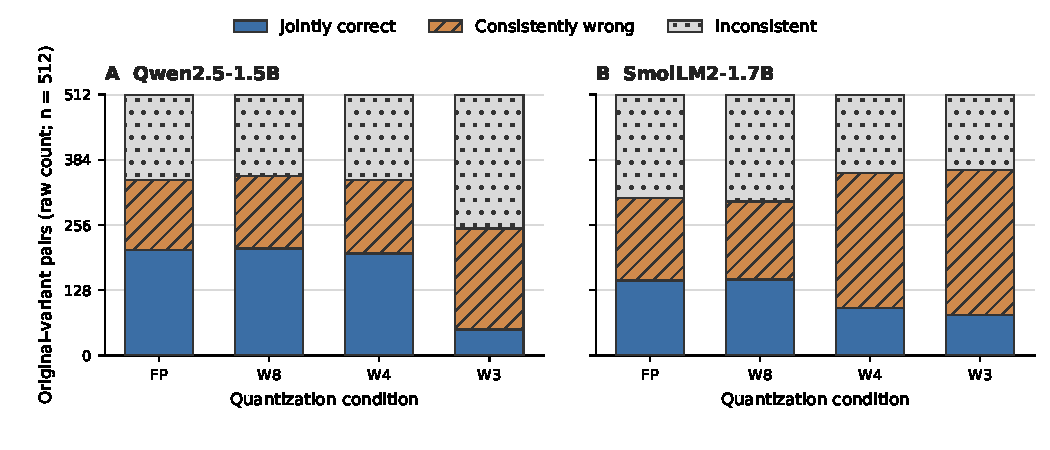
\includegraphics[width=\linewidth]{../figures/pilot/pilot_pair_outcomes.pdf}
\caption{Exploratory pilot outcomes for all 512 original-variant pairs per
model. Solid segments are jointly correct, hatched segments agree on a wrong
canonical option, and dotted segments disagree. These are descriptive raw
pair counts, not equal-base-weighted rates. BF16 is the reference; quantized
weights are dequantized for BF16 arithmetic.}
\label{fig:pilot}
\end{figure}

\section{Independent final results}
The independent evaluation contains 768 final bases and 384 structural-holdout
bases, rendered into 6,144 inputs per condition. Each model has 21 conditions:
BF16 and three RTN precisions, fifteen selected scale fits, the displayed-A
rule, and the calibration-only four-logit correction. No final outcome is
used for model, loss, checkpoint, or hyperparameter selection. Unless a split
is named, the following differences pool the 1,152 independent bases with
equal base weight. Reported seed ranges describe three individual fits;
they are not confidence intervals over training randomness.
Table~\ref{tab:final-contrasts} lists the pooled point estimates; the
released comparison files retain the corresponding base-bootstrap intervals
for the pooled data, each split, and each task family.

\begin{table}[t]
\centering\small
\caption{Paired-minus-augmented differences in percentage points over 1,152
bases per model. Singles denote held-out entity renaming/fact order;
compositions were withheld from fitting and selection. C is consistency,
J joint correctness, and W consistently wrong agreement. Seeds are distinct
fits evaluated on the same bases.}
\label{tab:final-contrasts}
\begin{tabular}{llrrrrr}
\toprule
 & & \multicolumn{3}{c}{Singles} & \multicolumn{2}{c}{Compositions}\\
Model & Seed & $\Delta C$ & $\Delta J$ & $\Delta W$ & $\Delta C$ & $\Delta J$\\
\midrule
Qwen & 17 & $-1.87$ & $+11.50$ & $-13.37$ & $+16.02$ & $+16.19$\\
Qwen & 29 & $-1.87$ & $+3.47$ & $-5.34$ & $+14.71$ & $+10.63$\\
Qwen & 43 & $-4.51$ & $+2.04$ & $-6.55$ & $+20.62$ & $+11.20$\\
Smol & 17 & $-8.77$ & $+4.25$ & $-13.02$ & $+9.11$ & $+9.81$\\
Smol & 29 & $-31.94$ & $-15.62$ & $-16.32$ & $-5.25$ & $-5.64$\\
Smol & 43 & $-13.06$ & $-1.65$ & $-11.41$ & $+8.16$ & $+4.56$\\
\bottomrule
\end{tabular}
\end{table}

\subsection{Qwen: correctness gains without primary consistency gains}
On held-out single transformations, paired calibration changes consistency
by $-1.87$, $-1.87$, and $-4.51$ percentage points versus same-seed augmented
KD (seeds 17, 29, and 43). The corresponding joint-correctness differences
are $+11.50$, $+3.47$, and $+2.04$ points, with base-bootstrap 95\% intervals
$[8.55,14.37]$, $[0.82,6.08]$, and $[-0.52,4.77]$.
Consistently wrong agreement falls by 5.34--13.37 points. Thus the primary
consistency outcome does not improve: more useful agreement partly replaces
wrong agreement, while total agreement is lower.

Compositions are a distinct secondary endpoint withheld from both updates
and development selection. Here consistency rises by 14.71--20.62 points
and joint correctness by 10.63--16.19 points. Every corresponding
per-fit interval lies above zero. However, consistently wrong composition
agreement also rises by 4.08 and 9.42 points at seeds 29 and 43; seed 17
changes it by $-0.17$ points with an interval spanning zero.
This is transfer of an invariance objective with a mixed error profile.
It is not uniformly beneficial consistency preservation.

The fidelity endpoint makes the distinction sharper. Relative to augmented
KD, paired calibration reduces held-out-single agreement with BF16 by
6.42--13.11 points, and composition agreement with BF16 by 3.39--12.63
points. The method can improve oracle correctness while moving away from
the full-precision teacher. These outcomes contradict an unqualified claim
that the paired loss preserves the teacher's behavior.

\subsection{Smol: the Qwen pattern does not transfer reliably}
Smol's held-out-single consistency falls by 8.77--31.94 points under paired
calibration. Joint correctness changes by $+4.25$, $-15.62$, and $-1.65$
points at seeds 17, 29, and 43. Consistently wrong agreement falls by
11.41--16.32 points, but this reduction does not ensure useful replacement:
at seed 29, correct agreement also falls substantially.
Composition consistency changes by $+9.11$, $-5.25$, and $+8.16$ points;
composition joint correctness changes by $+9.81$, $-5.64$, and $+4.56$.
Thus Qwen's positive composition result does not establish a benefit across
the two models and three fits. All fits completed the fixed 96 updates with
finite losses; no final outcome was used to replace the selected strength.
Across the three fits, held-out-single teacher fidelity falls by
12.72--33.20 points relative to augmented KD, and composition teacher
fidelity falls by 17.71--38.15 points. The loss is therefore not a reliable
teacher-preservation objective in either model.

The uncalibrated three-bit Smol model selects displayed A on 6,139 of 6,144
independent evaluation inputs (99.92\%), extending the pilot's all-A behavior
without claiming exact identity with a constant rule on the final data.
Figures~\ref{fig:final-primary}--\ref{fig:final-outcomes} show the 768-base
final split separately; the pooled contrasts above also include the 384
structural-holdout bases, whose results remain separately available.

\begin{figure}[t]
\centering
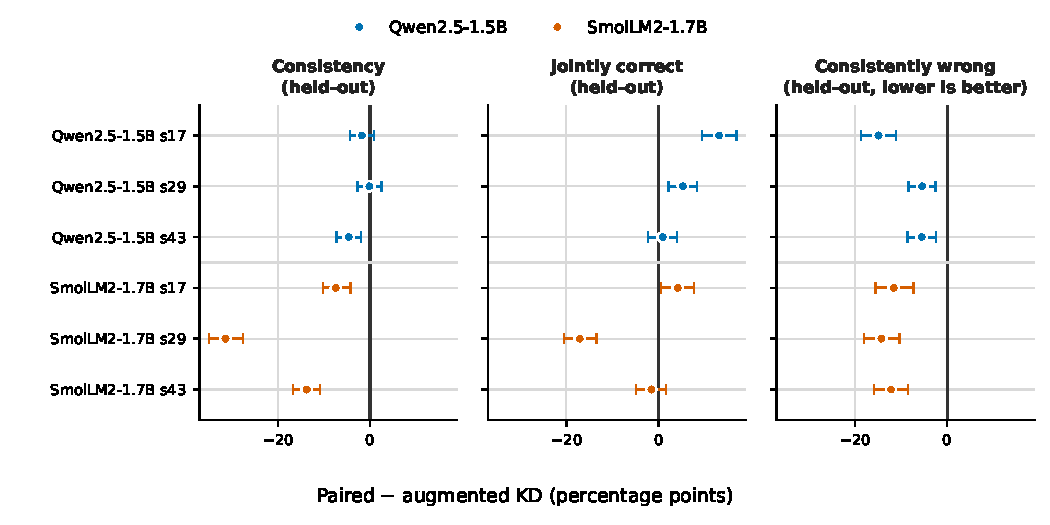
\includegraphics[width=\linewidth]{../figures/final/final_paired_vs_augmented_heldout.pdf}
\caption{Primary paired-minus-augmented contrasts on held-out single
transformations in the final split (768 bases per model). Each row is one
fit seed; horizontal intervals are percentile 95\% intervals from 1,000
paired base resamples. The three panels distinguish total agreement,
joint correctness, and consistently wrong agreement. Lower is better only
for the last panel. Intervals are conditional on each fit and unadjusted.}
\label{fig:final-primary}
\end{figure}

\begin{figure}[t]
\centering
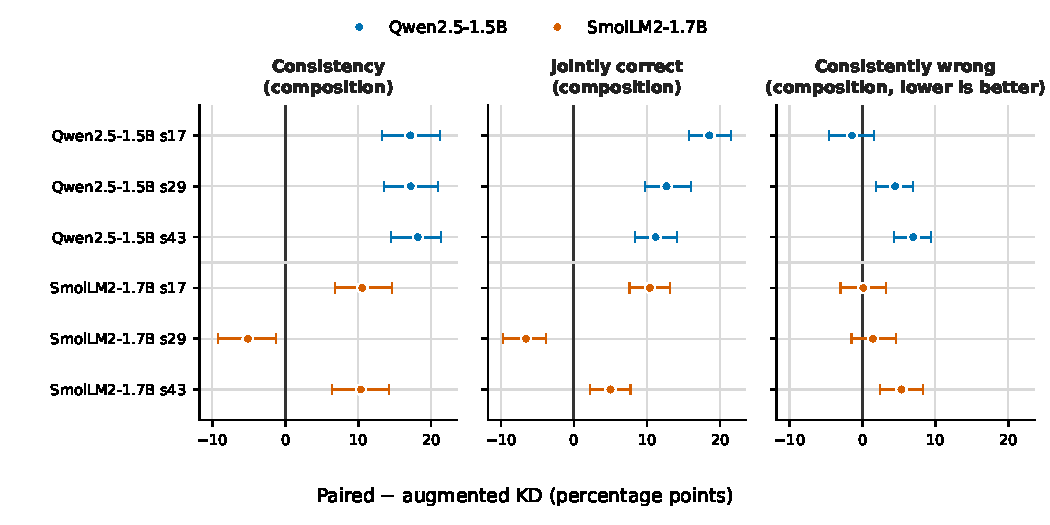
\includegraphics[width=\linewidth]{../figures/final/final_paired_vs_augmented_compositions.pdf}
\caption{Secondary contrasts on final-split compositions withheld from both
gradient updates and development selection (768 bases per model).
Conventions match Figure~\ref{fig:final-primary}. A consistency gain may
contain both more jointly correct and more consistently wrong pairs;
these components are shown separately.}
\label{fig:final-compositions}
\end{figure}

\begin{figure}[t]
\centering
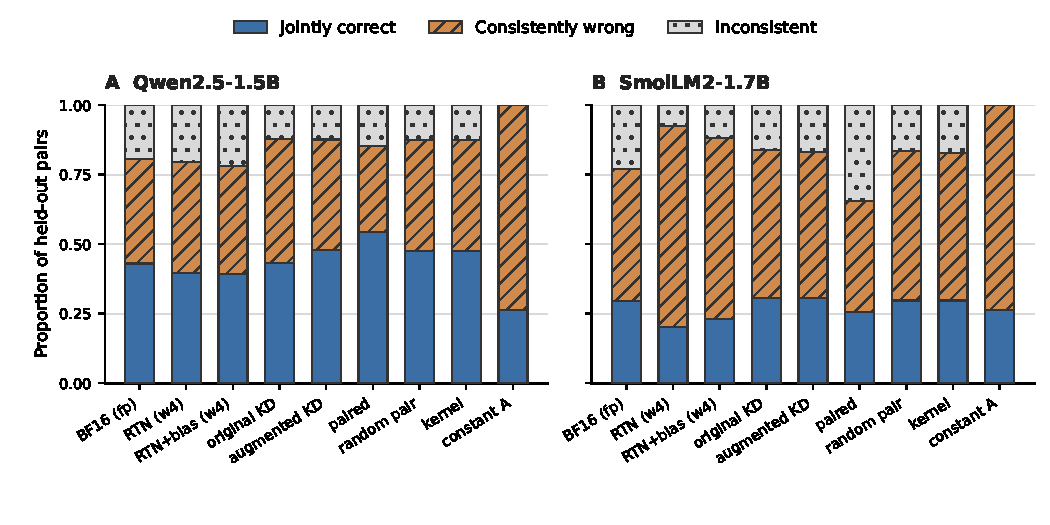
\includegraphics[width=\linewidth]{../figures/final/final_heldout_outcomes.pdf}
\caption{Absolute held-out-single outcomes on the final split. Each base
receives equal weight; learned conditions are descriptive means over seeds
17, 29, and 43, while untrained conditions have one result. Solid segments
are jointly correct, hatched segments consistently wrong, and dotted segments
disagree. The kernel condition is the matched cosine-Gram adaptation;
RTN+bias is the separate calibration-only four-logit rule. The constant-A
rule demonstrates that perfect consistency need not imply useful answers.}
\label{fig:final-outcomes}
\end{figure}

\clearpage
\section{Limitations and reproducibility}
This is a controlled study of two small instruction models on English
procedural multiple-choice problems. It does not establish performance on
natural-language paraphrases, free generation, long reasoning traces,
deployment kernels, or larger contemporary models. A higher consistency
score can result from a less informative predictor, including the displayed-A
rule. The full-precision teacher is also not an oracle, and enforcing
invariance can trade teacher fidelity against correctness.

The comparison isolates objectives within a signed RTN initialization and
a single-epoch scale schedule. We do not reproduce full KernelQuant or
benchmark against deployed AWQ/GPTQ pipelines. Their absence limits claims
about competitive quantization quality. The kernel adaptation is an
objective control, not a substitute for those complete systems.
The three-strength search does not equalize regularizer magnitudes, and an
individual seed's development results select the strength for all three fits.
This design measures repeatability of that selected recipe rather than
robustness under a multiseed selection procedure. An
unquantized scale-optimization control is absent. We therefore cannot attribute
an observed calibration benefit uniquely to compression or exclude generic
invariance fine-tuning as an explanation.
The four-logit diagnostic tests one fixed mean-drift correction, not every
possible position-bias explanation. Even an improvement over random pairing
does not establish a particular internal reasoning mechanism.
Equivalent Boolean functions or isomorphic graphs can cross the declared
exact-structure split boundary. The confidence intervals describe variation
across generated bases conditional on the fitted models and the fixed
prompt/format; they do not establish broad task-population guarantees.

The protocol, amendments, exact oracle structures, option maps, configurations,
per-input predictions, all development candidates, fit/timing records, and
plotting code accompany the reproducibility package. Upstream pretrained
weights and full-vocabulary teacher caches are not redistributed.
The released scale-calibration code and pinned original model revisions
allow fits to be regenerated. The draft separates the exposed pilot from
the independently reserved final split.

\section{Executed settings}
Table~\ref{tab:settings} records the common design. Model-specific strengths
were fixed from development before final inference. Both models completed
all 21 final conditions. Saved predictions reproduce all condition and
subgroup summaries and paired intervals in CPU replay; the offline suite
passes 106 tests.

The pinned model revisions are:
\begin{quote}\small
Qwen: \texttt{989aa7980e4cf806f80c7fef2b1adb7bc71aa306}\\
Smol: \texttt{31b70e2e869a7173562077fd711b654946d38674}
\end{quote}

\begin{table}[h]
\centering\small
\caption{Study settings and authoritative evidence}
\label{tab:settings}
\begin{tabular}{p{0.24\linewidth}p{0.45\linewidth}p{0.21\linewidth}}
\toprule
Item & Value & Evidence \\
\midrule
Models & Qwen2.5-1.5B-Instruct; SmolLM2-1.7B-Instruct
 & Pinned configs \\
Arithmetic & Two/three operations; five/six in structural holdout
 & Generator \\
Boolean & Three/four assignment variables; five in structural holdout
 & Generator \\
Graphs & DAGs with five--seven nodes; eight--ten in structural holdout
 & Generator \\
Bases per family & Calibration 128; development 128; pilot 64;
final 256; structural holdout 128 & Protocol and data manifests \\
Split seeds & 1108, 2108, 3108, 4108, 5108, respectively
 & Pinned configs \\
Quantizer & Signed grouped RTN; 128 input columns per row/group;
W4 calibration; BF16 forward arithmetic & Run manifests \\
Optimization & AdamW; 0.001 learning rate; 96 updates;
four bases/eight prompts per update & Fit manifests \\
Fit seeds & 17, 29, 43 & Fit manifests \\
Lambda candidates & 0.1, 1, 10; development-only selection
 & Frozen selections \\
Selected Qwen strengths & Paired 10; random pair 1; kernel 0.1
 & Qwen selection JSON \\
Selected Smol strengths & Paired 10; random pair 0.1; kernel 10
 & Smol selection JSON \\
Trainable scale deltas & Qwen 10,235,904; Smol 12,582,912
 & Fit manifests \\
Scoring & Official chat template; next-token A--D; batch 8;
maximum 1,024 prompt tokens without truncation & Scorer/configs \\
Intervals & 1,000 paired base resamples; seed 4108
 & Comparison JSON \\
Hardware/runtime & Radeon RX 9070 XT; ROCm PyTorch
2.12.0+rocm7.14.0; Transformers 4.57.1; Python 3.12
 & Run manifests \\
\bottomrule
\end{tabular}
\end{table}

\clearpage
\section*{Tool-use disclosure}
DeepSeek V4.1 Flash implemented the experimental code under Codex supervision.
Codex assisted with design, literature checking, execution, tests, and drafting.
The manuscript is a research draft rather than a record of peer review.

\begin{thebibliography}{11}
\bibitem{uda}
Qizhe Xie, Zihang Dai, Eduard Hovy, Minh-Thang Luong, and Quoc V. Le.
Unsupervised Data Augmentation for Consistency Training. NeurIPS, 2020.
\url{https://arxiv.org/abs/1904.12848}

\bibitem{augmix}
Dan Hendrycks et al. AugMix: A Simple Data Processing Method to Improve
Robustness and Uncertainty. arXiv:1912.02781v2, 2020.
\url{https://arxiv.org/html/1912.02781v2}

\bibitem{illusion}
Baha Rababah et al. The Illusion of Equivalency: Statistical Characterization
of Quantization Effects in LLMs. arXiv:2607.08734v2, 2026.
\url{https://arxiv.org/html/2607.08734v2}

\bibitem{fidelityq}
Chen et al. FidelityQ: Preserving Predictive Fidelity in Ultra-Low-Bit
Language Model Quantization. arXiv:2610.14934, 2026.
\url{https://arxiv.org/html/2610.14934}

\bibitem{dpq}
Yang et al. Target-Aware Calibration Data Selection for Preserving Uncertainty
in Quantized Language Models. Findings of EMNLP, 2026.
\url{https://aclanthology.org/2026.findings-emnlp.670/}

\bibitem{eaquant}
Yeji Kim, Mi-Young Kim, and Randy Goebel.
When Quantization Preserves Accuracy but Not Evidence: Explanation-Aware
Post-Training Quantization for Medical LLMs. EMNLP, pp.\ 41629--41651, 2026.
\url{https://aclanthology.org/2026.emnlp-main.1828/}

\bibitem{kernelquant}
Park et al. KernelQuant: Post-Training Quantization via Representation Kernel
Preservation. EMNLP, pp.\ 19833--19850, 2026.
\url{https://aclanthology.org/2026.emnlp-main.856/}

\bibitem{ostquant}
Hu et al. OSTQuant: Refining Large Language Model Quantization with Orthogonal
and Scaling Transformations for Better Distribution Fitting.
arXiv:2501.13987, 2025.
\url{https://arxiv.org/html/2501.13987}

\bibitem{roleq}
Johannes Knittel, Alec Helbling, and Hanspeter Pfister.
RoleQ: Role-Aligned Scales for Converting Language Models to Ternary.
arXiv:2610.21808, 2026.
\url{https://arxiv.org/html/2610.21808}

\bibitem{fptquant}
van Breugel et al. FPTQuant: Function-Preserving Transforms for LLM
Quantization. arXiv:2506.04985v2; ICML, 2026.
\url{https://arxiv.org/abs/2506.04985}

\bibitem{deceptive}
Fu et al. Quantized but Deceptive? A Multi-Dimensional Truthfulness Evaluation
of Quantized LLMs. EMNLP, pp.\ 30435--30458, 2025.
\url{https://aclanthology.org/2025.emnlp-main.1548/}

\bibitem{panels}
Ananto Nayan Bala. Does Quantization Change What Agreement Means? A Paired
Audit of Homogeneous LLM Panels. UncertaiNLP, 2026.
\url{https://aclanthology.org/2026.uncertainlp-main.37/}
\end{thebibliography}
\end{document}
